% Options for packages loaded elsewhere
% Options for packages loaded elsewhere
\PassOptionsToPackage{unicode}{hyperref}
\PassOptionsToPackage{hyphens}{url}
%
\documentclass[
  ignorenonframetext,
  aspectratio=169,
]{beamer}
\newif\ifbibliography
\usepackage{pgfpages}
\setbeamertemplate{caption}[numbered]
\setbeamertemplate{caption label separator}{: }
\setbeamercolor{caption name}{fg=normal text.fg}
\beamertemplatenavigationsymbolsempty
% remove section numbering
\setbeamertemplate{part page}{
  \centering
  \begin{beamercolorbox}[sep=16pt,center]{part title}
    \usebeamerfont{part title}\insertpart\par
  \end{beamercolorbox}
}
\setbeamertemplate{section page}{
  \centering
  \begin{beamercolorbox}[sep=12pt,center]{section title}
    \usebeamerfont{section title}\insertsection\par
  \end{beamercolorbox}
}
\setbeamertemplate{subsection page}{
  \centering
  \begin{beamercolorbox}[sep=8pt,center]{subsection title}
    \usebeamerfont{subsection title}\insertsubsection\par
  \end{beamercolorbox}
}
% Prevent slide breaks in the middle of a paragraph
\widowpenalties 1 10000
\raggedbottom
\usepackage{iftex}
\ifPDFTeX
  \usepackage[T1]{fontenc}
  \usepackage[utf8]{inputenc}
  \usepackage{textcomp} % provide euro and other symbols
\else % if luatex or xetex
  \usepackage{unicode-math} % this also loads fontspec
  \defaultfontfeatures{Scale=MatchLowercase}
  \defaultfontfeatures[\rmfamily]{Ligatures=TeX,Scale=1}
\fi
\usepackage{lmodern}

\ifPDFTeX\else
  % xetex/luatex font selection
\fi
% Use upquote if available, for straight quotes in verbatim environments
\IfFileExists{upquote.sty}{\usepackage{upquote}}{}
\IfFileExists{microtype.sty}{% use microtype if available
  \usepackage[]{microtype}
  \UseMicrotypeSet[protrusion]{basicmath} % disable protrusion for tt fonts
}{}
\makeatletter
\@ifundefined{KOMAClassName}{% if non-KOMA class
  \IfFileExists{parskip.sty}{%
    \usepackage{parskip}
  }{% else
    \setlength{\parindent}{0pt}
    \setlength{\parskip}{6pt plus 2pt minus 1pt}}
}{% if KOMA class
  \KOMAoptions{parskip=half}}
\makeatother


\usepackage{longtable,booktabs,array}
\usepackage{calc} % for calculating minipage widths
\usepackage{caption}
% Make caption package work with longtable
\makeatletter
\def\fnum@table{\tablename~\thetable}
\makeatother
\usepackage{graphicx}
\makeatletter
\newsavebox\pandoc@box
\newcommand*\pandocbounded[1]{% scales image to fit in text height/width
  \sbox\pandoc@box{#1}%
  \Gscale@div\@tempa{\textheight}{\dimexpr\ht\pandoc@box+\dp\pandoc@box\relax}%
  \Gscale@div\@tempb{\linewidth}{\wd\pandoc@box}%
  \ifdim\@tempb\p@<\@tempa\p@\let\@tempa\@tempb\fi% select the smaller of both
  \ifdim\@tempa\p@<\p@\scalebox{\@tempa}{\usebox\pandoc@box}%
  \else\usebox{\pandoc@box}%
  \fi%
}
% Set default figure placement to htbp
\def\fps@figure{htbp}
\makeatother





\setlength{\emergencystretch}{3em} % prevent overfull lines

\providecommand{\tightlist}{%
  \setlength{\itemsep}{0pt}\setlength{\parskip}{0pt}}



 


% nf-macros.tex — visual building blocks for "Metodi Statistici per la Neuropsicologia Forense"
% Adapted from the Time Management deck (tm-macros.tex); loads unipdwarsawstyle.sty first.

% ---------------------------------------------------------
% FONTS, ICONS, LIBRARIES
% ---------------------------------------------------------
\usepackage{unipdwarsawstyle}
\usepackage[sfdefault]{FiraSans}
\usepackage{fontawesome5}
\usetikzlibrary{arrows.meta,positioning,calc,fit,backgrounds,shapes.geometric}

% ---------------------------------------------------------
% IMAGE HEIGHT CAP — 16:9 frames are shorter than the old 4:3 ones, so images sized
% by width can run off the bottom. Every \includegraphics taller than \nfmaxheight
% is scaled down (aspect ratio kept); unsized markdown images use the same limit.
% ---------------------------------------------------------
\newlength{\nfmaxheight}
\AtBeginDocument{\setlength{\nfmaxheight}{0.74\textheight}}
\makeatletter
\newsavebox\nf@imgbox
\let\nf@includegraphics\includegraphics
\renewcommand*\includegraphics[2][]{%
  \sbox\nf@imgbox{\nf@includegraphics[#1]{#2}}%
  \ifdim\dimexpr\ht\nf@imgbox+\dp\nf@imgbox\relax>\nfmaxheight
    \resizebox{!}{\nfmaxheight}{\usebox\nf@imgbox}%
  \else\usebox\nf@imgbox\fi}
% unsized markdown images: fit within \linewidth and \nfmaxheight
\renewcommand*\pandocbounded[1]{%
  \sbox\nf@imgbox{#1}%
  \Gscale@div\@tempa{\nfmaxheight}{\dimexpr\ht\nf@imgbox+\dp\nf@imgbox\relax}%
  \Gscale@div\@tempb{\linewidth}{\wd\nf@imgbox}%
  \ifdim\@tempb\p@<\@tempa\p@\let\@tempa\@tempb\fi
  \ifdim\@tempa\p@<\p@\scalebox{\@tempa}{\usebox\nf@imgbox}\else\usebox\nf@imgbox\fi}
\makeatother

% ---------------------------------------------------------
% PALETTE — structure is UniPD crimson/gold (from the style file)
% ---------------------------------------------------------
\definecolor{nfInk}{HTML}{243447}      % dark text
\definecolor{nfPoll}{HTML}{5B3F9E}     % Wooclap
\definecolor{nfPadlet}{HTML}{B8860B}   % Padlet
\definecolor{nfGrey}{HTML}{8A94A0}

% ---------------------------------------------------------
% GLOBAL LOOK
% ---------------------------------------------------------
\hyphenpenalty=10000 \exhyphenpenalty=10000
\setbeamertemplate{headline}{}
\setbeamercolor{background canvas}{bg=white}
\setbeamercolor{normal text}{fg=nfInk}
\setbeamerfont{frametitle}{size=\large,series=\bfseries}
\setbeamertemplate{footline}{%
  \hfill{\color{nfGrey}\tiny\insertframenumber}\hspace*{4mm}\vspace*{2mm}}
\setbeamertemplate{itemize item}{\color{unipdCrimson}\raisebox{0.15ex}{\scriptsize\faCircle}}

% ---------------------------------------------------------
% ICON ROW — icon in a crimson disc + text
%   \iconrow{\faVideo}{Text}
% ---------------------------------------------------------
\newcommand{\iconrow}[2]{%
  \par\noindent
  \begin{minipage}[c]{0.9cm}\centering
    \tikz\node[circle, fill=unipdCrimson, text=white, minimum size=7mm, inner sep=0pt]{\small #1};
  \end{minipage}%
  \begin{minipage}[c]{\dimexpr\linewidth-0.9cm\relax}\small #2\end{minipage}\par\vspace{5pt}}

% ---------------------------------------------------------
% ACTIVITIES — real QR code and join code
% ---------------------------------------------------------
\newcommand{\timer}[1]{%
  \tikz[baseline=(t.base)]\node[fill=unipdCrimson, text=white, rounded corners=6pt,
    font=\scriptsize\bfseries, inner sep=3pt] (t) {\faIcon{stopwatch}\ #1};}

%   \qrbox{colour}{Figures/qr.png}{code or empty}
\newcommand{\qrbox}[3]{%
  \begin{tikzpicture}
    \node[draw=#1, line width=1.2pt, rounded corners=5pt, inner sep=5pt, fill=white] (q)
      {\includegraphics[width=3.4cm]{#2}};
    \if\relax\detokenize{#3}\relax\else
      \node[below=3pt of q, font=\small\bfseries\color{#1}] {codice: #3};
    \fi
  \end{tikzpicture}}

%   \wooclapslot{tipo}{domanda}{istruzioni}{minuti o vuoto}{Figures/qr.png}{codice}
\newcommand{\wooclapslot}[6]{%
  \begin{columns}[c]
    \begin{column}{0.56\textwidth}
      {\color{nfPoll}\small\faPoll\ \textbf{WOOCLAP}\,·\,#1}%
      \if\relax\detokenize{#4}\relax\else\hfill\timer{#4}\fi\par\vspace{8pt}
      {\LARGE\bfseries\color{nfInk}#2\par}\vspace{10pt}
      {\small\color{nfInk}#3\par}
    \end{column}
    \begin{column}{0.40\textwidth}\centering\qrbox{nfPoll}{#5}{#6}\end{column}
  \end{columns}}

%   \padletslot{tipo}{domanda}{istruzioni}{minuti o vuoto}{Figures/qr.png}
\newcommand{\padletslot}[5]{%
  \begin{columns}[c]
    \begin{column}{0.56\textwidth}
      {\color{nfPadlet}\small\faStickyNote\ \textbf{PADLET}\,·\,#1}%
      \if\relax\detokenize{#4}\relax\else\hfill\timer{#4}\fi\par\vspace{8pt}
      {\LARGE\bfseries\color{nfInk}#2\par}\vspace{10pt}
      {\small\color{nfInk}#3\par}
    \end{column}
    \begin{column}{0.40\textwidth}\centering\qrbox{nfPadlet}{#5}{}\end{column}
  \end{columns}}

% ---------------------------------------------------------
% TITLE SLIDE — use on a  ## {.plain}  frame:   \nftitleslide{2 · Cornice teorica}
% ---------------------------------------------------------
\newcommand{\nftitleslide}[1]{%
  \begin{tikzpicture}[remember picture, overlay]
    \fill[unipdCrimson] (current page.north west) rectangle ([xshift=0.58\paperwidth]current page.south west);
    \fill[unipdGold] ([xshift=0.58\paperwidth]current page.north west) rectangle ([xshift=0.585\paperwidth]current page.south west);
  \end{tikzpicture}%
  \begin{columns}[c]
    \begin{column}{0.55\textwidth}
      \color{white}
      {\small\color{unipdGold}\MakeUppercase{#1}\par}\vspace{6pt}
      {\fontsize{22}{27}\selectfont\bfseries Metodi Statistici per la Neuropsicologia Forense\par}\vspace{22pt}
      {\small\bfseries Giorgio Arcara\par}
      {\scriptsize Università di Padova\\ IRCCS San Camillo, Venezia\par}
    \end{column}
    \begin{column}{0.40\textwidth}\centering
      
\includegraphics[width=0.85\linewidth]{Figures/LogoSanCamilloIRCCS_Unipd_alpha.png}\par\vspace{14pt}
      
\includegraphics[height=0.55cm]{Figures/CC_license_3_0.png}
    \end{column}
  \end{columns}}

% ---------------------------------------------------------
% SECTION DIVIDER — built automatically from each "# Section" heading
% (YAML: section-titles: false, so Quarto does not add its own)
% ---------------------------------------------------------
\AtBeginSection{%
  \begin{frame}[plain]
    \begin{tikzpicture}[remember picture, overlay]
      \fill[unipdCrimson] (current page.north west) rectangle ([xshift=3mm]current page.south west);
      \fill[unipdGold] ([xshift=3mm]current page.north west) rectangle ([xshift=3.6mm]current page.south west);
      \node[anchor=north west, font=\scriptsize\color{nfGrey}, inner sep=0pt]
        at ([xshift=8mm,yshift=-5mm]current page.north west)
        {METODI STATISTICI PER LA NEUROPSICOLOGIA FORENSE};
    \end{tikzpicture}
    \vfill
    \begin{center}
      {\fontsize{26}{32}\selectfont\bfseries\color{unipdCrimson}\insertsectionhead\par}
    \end{center}
    \vfill
  \end{frame}}

% ---------------------------------------------------------
% TAKEAWAY strip at the bottom of the slide
% ---------------------------------------------------------
\newcommand{\takeaway}[1]{%
  \begin{tikzpicture}[remember picture, overlay]
    \node[anchor=south west, fill=unipdCream!70, text=nfInk, font=\scriptsize,
          inner xsep=6pt, inner ysep=3pt, rounded corners=2pt, text width=0.84\paperwidth]
      at ([xshift=5mm,yshift=4mm]current page.south west)
      {\textcolor{unipdCrimson}{\faKey}\ \textbf{In sintesi:} #1};
  \end{tikzpicture}}
\usepackage{booktabs}
\usepackage{array}
% same as \nftitleslide in nf-macros.tex, with the author line as first argument
\newcommand{\nftitleslideauthors}[2]{%
  \begin{tikzpicture}[remember picture, overlay]
    \fill[unipdCrimson] (current page.north west) rectangle ([xshift=0.58\paperwidth]current page.south west);
    \fill[unipdGold] ([xshift=0.58\paperwidth]current page.north west) rectangle ([xshift=0.585\paperwidth]current page.south west);
  \end{tikzpicture}%
  \begin{columns}[c]
    \begin{column}{0.55\textwidth}
      \color{white}
      {\small\color{unipdGold}\MakeUppercase{#2}\par}\vspace{6pt}
      {\fontsize{22}{27}\selectfont\bfseries Metodi Statistici per la Neuropsicologia Forense\par}\vspace{22pt}
      {\small\bfseries #1\par}
      {\scriptsize Università di Padova\\ IRCCS San Camillo, Venezia\par}
    \end{column}
    \begin{column}{0.40\textwidth}\centering
      
\includegraphics[width=0.85\linewidth]{Figures/LogoSanCamilloIRCCS_Unipd_alpha.png}\par\vspace{14pt}
      
\includegraphics[height=0.55cm]{Figures/CC_license_3_0.png}
    \end{column}
  \end{columns}}
\makeatletter
\@ifpackageloaded{caption}{}{\usepackage{caption}}
\AtBeginDocument{%
\ifdefined\contentsname
  \renewcommand*\contentsname{Table of contents}
\else
  \newcommand\contentsname{Table of contents}
\fi
\ifdefined\listfigurename
  \renewcommand*\listfigurename{List of Figures}
\else
  \newcommand\listfigurename{List of Figures}
\fi
\ifdefined\listtablename
  \renewcommand*\listtablename{List of Tables}
\else
  \newcommand\listtablename{List of Tables}
\fi
\ifdefined\figurename
  \renewcommand*\figurename{Figure}
\else
  \newcommand\figurename{Figure}
\fi
\ifdefined\tablename
  \renewcommand*\tablename{Table}
\else
  \newcommand\tablename{Table}
\fi
}
\@ifpackageloaded{float}{}{\usepackage{float}}
\floatstyle{ruled}
\@ifundefined{c@chapter}{\newfloat{codelisting}{h}{lop}}{\newfloat{codelisting}{h}{lop}[chapter]}
\floatname{codelisting}{Listing}
\newcommand*\listoflistings{\listof{codelisting}{List of Listings}}
\makeatother
\makeatletter
\makeatother
\makeatletter
\@ifpackageloaded{caption}{}{\usepackage{caption}}
\@ifpackageloaded{subcaption}{}{\usepackage{subcaption}}
\makeatother

\usepackage{bookmark}
\IfFileExists{xurl.sty}{\usepackage{xurl}}{} % add URL line breaks if available
\urlstyle{same}
\hypersetup{
  pdfauthor={Giorgio Arcara, Sara Lago},
  hidelinks,
  pdfcreator={LaTeX via pandoc}}


\author{Giorgio Arcara, Sara Lago}
\date{}

\begin{document}


\begin{frame}[plain]{}
\phantomsection\label{section}
\nftitleslideauthors{Giorgio Arcara, Sara Lago}{3a · Affidabilità (teoria)}
\end{frame}

\begin{frame}{Validità e affidabilità (brevi definizioni)}
\phantomsection\label{validituxe0-e-affidabilituxe0-brevi-definizioni}
La \textbf{validità} è la qualità di un test di misurare effettivamente
il costrutto che vuole misurare.

L' \textbf{affidabilità} indica la precisione di un test.
\end{frame}

\section{Affidabilità}\label{affidabilituxe0}

\begin{frame}{Affidabilità/precisione}
\phantomsection\label{affidabilituxe0precisione}
L'\textbf{Affidabilità} è la qualità di un test di fornire punteggi
consistenti in diverse misurazioni: può essere intesa come la
\textbf{precisione} di un test.

Come per la validità, gli \emph{Standards} (AERA, APA, \& NCME, 2014)
trattano l'affidabilità come un \textbf{principio unitario} ---
l'ombrello ``affidabilità/precisione'' --- di cui i ``tipi'' che seguono
sono sfaccettature diverse, non categorie separate.
\end{frame}

\begin{frame}{Tipi Affidabilità}
\phantomsection\label{tipi-affidabilituxe0}
\begin{itemize}
\tightlist
\item
  Affidabilità inter-rater
\item
  Affidabilità test-retest
\item
  Affidabilità split-half
\item
  Consistenza Interna
\end{itemize}

Esistono diverse classificazioni di affidabilità. Questa che sto
utilizzando è una delle possibili.
\end{frame}

\begin{frame}{Valori desiderabili}
\phantomsection\label{valori-desiderabili}
Spesso le misure di affidabilità sono associate a numeri. Le slide
seguenti ipotizzerò dei valori desiderabili di affidabilità che un test
dovrebbe avere.

È importante che questi sono valori ``indicativi'' e non esistono reali
valori considerati come standard nella letteratura. Per tale ragione
spesso circolano test con valori ben più bassi di quelli desiderabili.
\end{frame}

\begin{frame}{Inter-rater agreement 1/2}
\phantomsection\label{inter-rater-agreement-12}
\textbf{Inter-rater agreement} (affidabilità inter-rater): è una misura
della consistenza con cui diversi esaminatori valutano la stessa
prestazione dello stesso paziente.
\end{frame}

\begin{frame}{Attività (Wooclap)}
\phantomsection\label{attivituxe0-wooclap}
\wooclapslot{Domanda}{Secondo te, quali fattori riguardanti un test possono influenzare il suo inter-rater agreement?}{Andate su \href{https://www.wooclap.com}{\underline{wooclap.com}} e inserite il codice \textbf{SOZZBAQ}, oppure inquadrate il QR code.}{}{Figures/wooclap_qr_code_SOZZBAQ.png}{SOZZBAQ}
\end{frame}

\begin{frame}{Inter-rater agreement 2/2}
\phantomsection\label{inter-rater-agreement-22}
È legata alla chiarezza delle istruzioni su come attribuire i punteggi e
alla complessità dei comportamenti osservati nel test --- ed è collegata
al concetto di \textbf{oggettività} del test (vedi Cornice teorica).

Esistono vari modi di calcolarla. Nel metodo più diffuso è espressa da
un coefficiente, l'intraclass correlation (ICC) --- una
\textbf{famiglia} di coefficienti --- che varia tra 0 e 1, dove 0 indica
completa inconsistenza tra i punteggi e 1 indica assoluta consistenza
tra i punteggi di due o più esaminatori.

Valori maggiori a 0.60 sono desiderabili (Cicchetti \& Sparrow, 1981;
Fastenau et al., 1996).
\end{frame}

\begin{frame}{Affidabilità test-retest 1/8}
\phantomsection\label{affidabilituxe0-test-retest-18}
\textbf{Affidabilità test-retest}: la consistenza dei punteggi ottenuti
dalle stesse persone in due occasioni diverse, assumendo che non ci sia
stato un cambiamento \emph{reale} nel costrutto misurato e che le
condizioni di somministrazione siano comparabili.

In genere è espressa da un coefficiente di correlazione che varia tra -1
e 1, ma può essere anche espressa dal coefficiente ICC (lo stesso usato
per Inter-rater agreement).

valori maggiori a 0.70 sono desiderabili
\end{frame}

\begin{frame}{Affidabilità test-retest 2/8}
\phantomsection\label{affidabilituxe0-test-retest-28}
Nota che l'affidabilità test-retest è sempre valutate con uno specifico
intervallo (es. 1 mese). Per tale ragioni esistono infinite possibili
affidabilità test-retest, dal momento che questo valore potrebbe variare
a seconda dell'intervallo.

Generalmente, più corto è l'intervallo, più è probabile sia alta
l'affidabilità test-retest.
\end{frame}

\begin{frame}{Affidabilità test-retest 3/8}
\phantomsection\label{affidabilituxe0-test-retest-38}
\begin{columns}
\column{0.8\textwidth}
\small
\textbf{Se misurata con correlazione, l'affidabilità test-retest \textbf{non indica la stabilità del punteggio dei test nel tempo, o la possibilità di usarlo per fare valutazioni nel tempo.}} 

\column{0.2\textwidth}
\begin{figure}
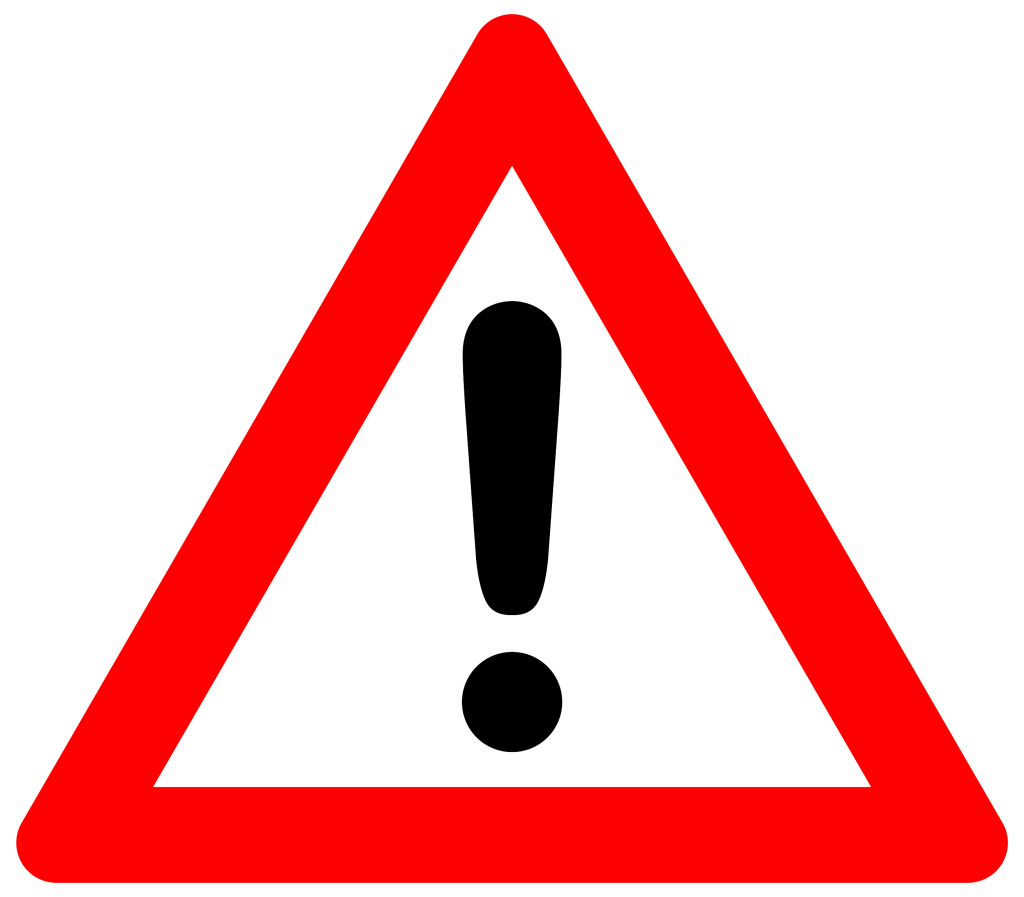
\includegraphics[scale=0.05]{Figures/triangle.png}
\end{figure}
\end{columns}

La correlazione cattura infatti solo la \textbf{consistenza relativa}
(l'ordine relativo delle persone si mantiene), non un accordo assoluto
sui valori --- per questo va sempre affiancata da un'analisi dei
cambiamenti sistematici (es. confronto delle medie; vedi Arcara \&
Bambini, 2016).
\end{frame}

\begin{frame}{Affidabilità test-retest 4/8}
\phantomsection\label{affidabilituxe0-test-retest-48}
Se ripeto la valutazione con lo stesso test alla stessa persona a
distanza di un tempo x, posso essere ragionevolmente sicura che il
punteggio al test rifletta le sue reali abilità cognitive, e sia
influenzato solo in misura trascurabile dalle circostanze della
somministrazione.
\end{frame}

\begin{frame}{Affidabilità test-retest 5/8}
\phantomsection\label{affidabilituxe0-test-retest-58}
La teoria classica dei test postula che il punteggio osservato sia
composto da punteggio vero + errore.

\begin{center}
$X = T + E$
\end{center}

\(X\) = punteggio osservato

\(T\) = punteggio vero

\(E\) = errore

\vspace{1em}

L'affidabilità test-retest cerca di quantificare l'errore legato a
misurazioni ripetute di un test.
\end{frame}

\begin{frame}{Esempio: confronto tra test con alta vs bassa affidabilità
test-retest}
\phantomsection\label{esempio-confronto-tra-test-con-alta-vs-bassa-affidabilituxe0-test-retest}
\begin{columns}[T]
\column{0.48\textwidth}\centering
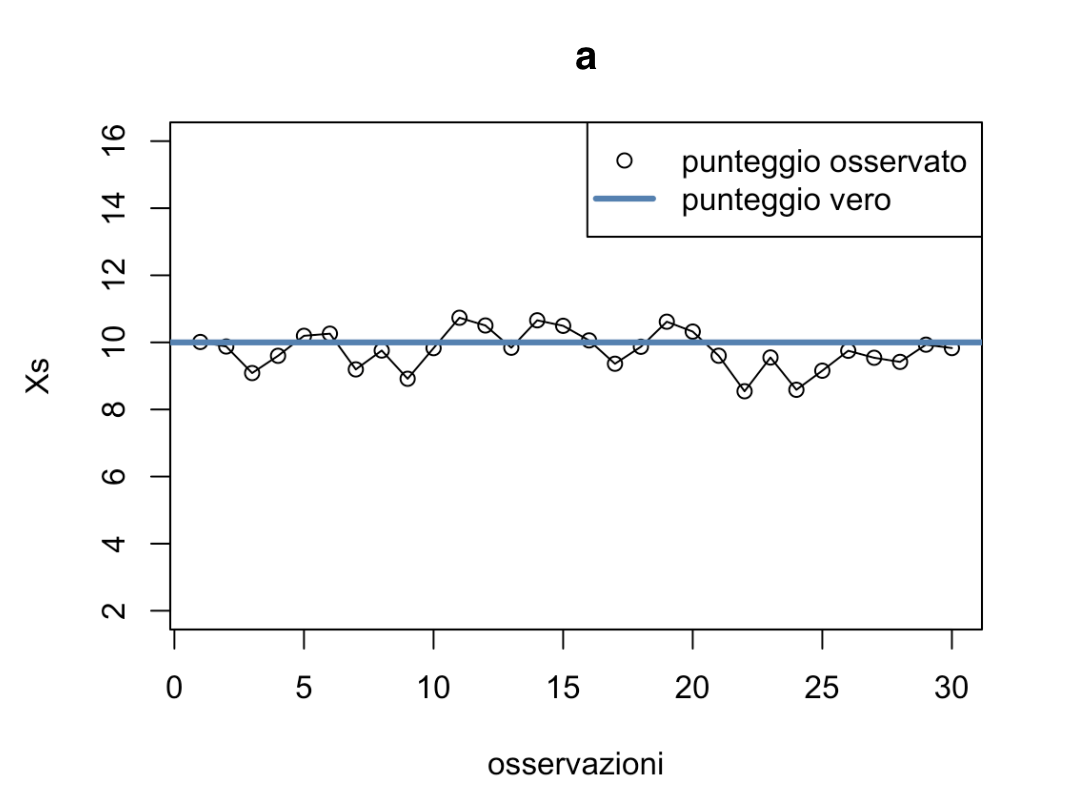
\includegraphics[height=0.58\textheight]{Figures/test_retest_alta_vs_bassa_a.png}
\column{0.48\textwidth}\centering
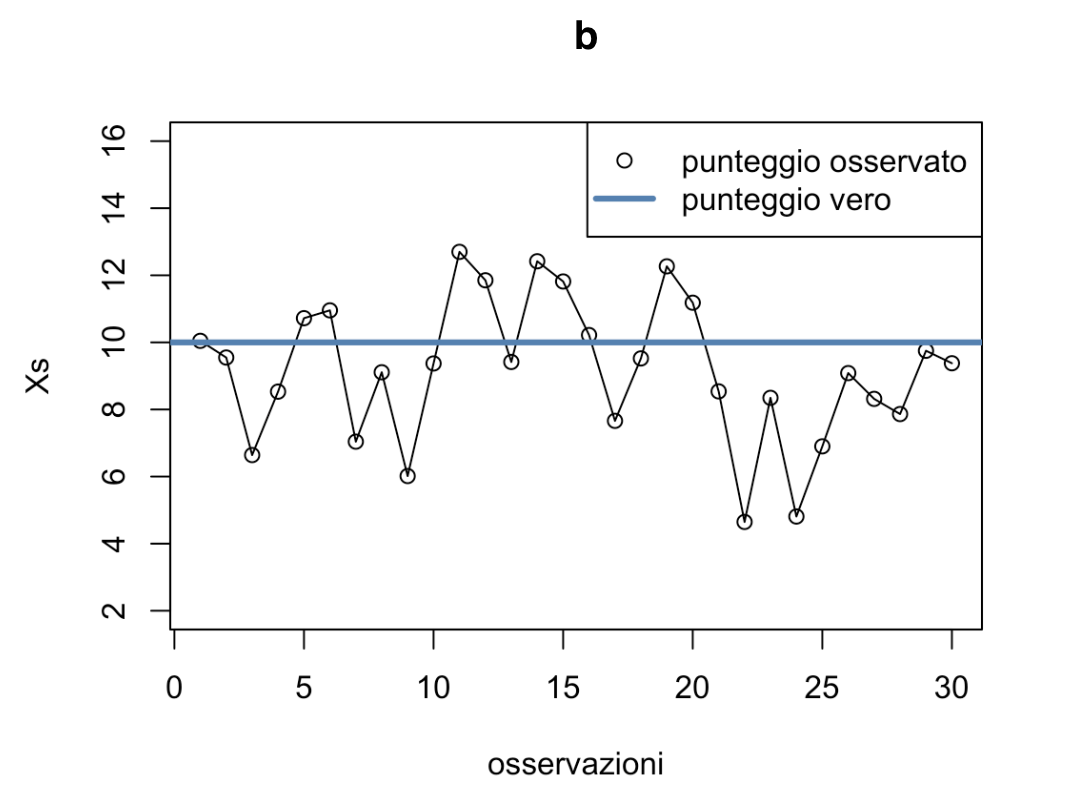
\includegraphics[height=0.58\textheight]{Figures/test_retest_alta_vs_bassa_b.png}
\end{columns}
\vspace{6pt}
\centering\textbf{Qual è la differenza tra i due grafici? Quale dei due corrisponde ad alta affidabilità test-retest e perché?}
\end{frame}

\begin{frame}{Affidabilità test-retest 6/8}
\phantomsection\label{affidabilituxe0-test-retest-68}
Quando è usata la correlazione come misura, i punteggi potrebbero avere
un'affidabilità test-retest (correlazione) di 0.98, ma essere poco
stabili perché soggetti a \emph{variazioni sistematiche}.

\pause

\textbf{Problema}: l'affidabilità test retest calcolata con correlazione
non tiene conto delle \textbf{variazioni sistematiche} nella
performance, cioè quei \textbf{cambiamenti non casuali} tra i punteggi
al test e al retest che si verificano per ogni individuo: l'effetto
pratica e regressione verso la media. Il cambiamento esiste, ma questa
concettualizzazione dell'affidabilità test retest non la prevede!
\end{frame}

\begin{frame}{Affidabilità test-retest 7/8}
\phantomsection\label{affidabilituxe0-test-retest-78}
La teoria classica dei test postula che il punteggio osservato sia
composto da punteggio vero + errore.

\begin{center}
$X = T + E$
\end{center}

\(X\) = punteggio osservato

\(T\) = punteggio vero

\(E\) = errore

\vspace{1em}

L'affidabilità test-retest cerca di quantificare l'errore legato a
misurazioni ripetute di un test.

Esistono diverse fonti di errore: casuale e sistematico. In questo caso
stiamo cercando di quantificare l'errore \textbf{casuale} (dovuto a
circostanze legate alla somministrazione).
\end{frame}

\begin{frame}{Affidabilità test-retest 8/8}
\phantomsection\label{affidabilituxe0-test-retest-88}
Visto che questa definizione non tiene conto dei cambiamenti
sistematici, oltre a considerare il valore di affidabilità test-retest
bisognerebbe sempre affiancare anche un'analisi di differenza delle
medie (t-test o altri metodi, es. APACS; Arcara \& Bambini, 2016) per
verificare che i punteggi al test e al retest siano (o meno)
effettivamente diversi.
\end{frame}

\begin{frame}{Domanda}
\phantomsection\label{domanda}
\vfill
\begin{center}
{\LARGE\bfseries Esistono casi nei quali è necessario capire se la performance cognitiva di una persona è cambiata nel tempo?\par}
\vspace{1.2em}
{\LARGE\bfseries Come fareste a valutare il cambiamento?\par}
\end{center}
\vfill
\end{frame}

\begin{frame}{Esempio}
\phantomsection\label{esempio}
AD è una donna di 63 anni che soffre di morbo di Parkinson. Per mitigare
i sintomi motori, le viene proposto un intervento per installare un
dispositivo DBS. Prima di sottoporsi all'intervento, svolge una
valutazione neuropsicologica di routine per monitorare i sintomi
cognitivi.

Un mese dopo l'intervento, i familiari di AD notano un repentino
peggioramento delle sue abilità cognitive. Sono convinti che questo
dipenda dall'intervento e non dal normale progredire della malattia, e
vogliono intentare una causa per danni. Pertanto, incaricano un
consulente di parte di dimostrarlo. Basandosi sull'ultima valutazione,
il consulente ne effettua un'altra usando gli stessi test.

Di seguito i punteggi.
\end{frame}

\begin{frame}{Esempio: punteggi di AD 1/2}
\phantomsection\label{esempio-punteggi-di-ad-12}
\begin{center}
\tiny\setlength{\tabcolsep}{2.5pt}\renewcommand{\arraystretch}{1.05}
\begin{tabular}{>{\raggedright\arraybackslash}p{1.85cm} >{\raggedright\arraybackslash}p{2.95cm} >{\centering\arraybackslash}p{1.15cm} >{\centering\arraybackslash}p{1.15cm} >{\centering\arraybackslash}p{0.75cm} >{\centering\arraybackslash}p{0.85cm} >{\centering\arraybackslash}p{1.45cm} >{\centering\arraybackslash}p{1.12cm} >{\centering\arraybackslash}p{1.12cm} >{\centering\arraybackslash}p{1.0cm}}
\toprule
\textbf{Dominio} & \textbf{Test} & \textbf{Prima valutazione: grezzo (corretto)} & \textbf{Seconda valutazione: grezzo (corretto)} & \textbf{Cut-off} & \textbf{Punteggio massimo} & \textbf{Soglie cambiamento significativo (solo APACS)} & \textbf{Prima valutazione (\%)} & \textbf{Seconda valutazione (\%)} & \textbf{Differenza \% (seconda $-$ prima)} \\
\midrule
Pragmatica & APACS interview & 34\textsuperscript{*} & 31\textsuperscript{*} & 42 & 44 & No thresholds available & 77.27 & 70.45 & $-$6.82 \\
 & APACS description & 46 & 41\textsuperscript{*}\textsuperscript{°} & 45 & 48 & 44---no upper threshold & 95.83 & 85.42 & $-$10.42 \\
 & APACS narratives & 47 & 39\textsuperscript{*}\textsuperscript{°} & 47 & 56 & 52---no upper threshold & 83.93 & 69.64 & $-$14.29 \\
 & APACS figurative language 1 & 14 & 14\textsuperscript{°} & 13 & 15 & 14---no upper threshold & 93.33 & 93.33 & 0 \\
 & APACS humor & 5 & 7\textsuperscript{°} & 4 & 7 & 5--6 & 71.43 & 100 & +28.57 \\
 & APACS figurative language 2 & 13\textsuperscript{*} & 10\textsuperscript{*} & 21 &  & No thresholds available & 43.33 & 33.33 & $-$10 \\
 & APACS pragmatic comprehension composite & 0.73\textsuperscript{*} & 0.74\textsuperscript{*} & 0.78 & 1 & 0.72--0.84 & 73 & 74 & +1 \\
 & APACS pragmatic production composite & 0.87\textsuperscript{*} & 0.78\textsuperscript{*}\textsuperscript{°} & 0.95 & 1 & 0.87--0.92 & 87 & 78 & $-$9 \\
 & APACS total composite & 0.8\textsuperscript{*} & 0.76\textsuperscript{*}\textsuperscript{°} & 0.88 & 1 & 0.82--0.88 & 80 & 76 & $-$4 \\
\bottomrule
\end{tabular}
\end{center}
\vspace{-0.8em}
{\tiny \textsuperscript{*} = performance deficitaria; \textsuperscript{°} = cambiamento significativo. Adattata da Lago et al. (2022).\par}
\end{frame}

\begin{frame}{Esempio: punteggi di AD 2/2}
\phantomsection\label{esempio-punteggi-di-ad-22}
\begin{center}
\tiny\setlength{\tabcolsep}{2.5pt}\renewcommand{\arraystretch}{1.05}
\begin{tabular}{>{\raggedright\arraybackslash}p{1.85cm} >{\raggedright\arraybackslash}p{2.95cm} >{\centering\arraybackslash}p{1.15cm} >{\centering\arraybackslash}p{1.15cm} >{\centering\arraybackslash}p{0.75cm} >{\centering\arraybackslash}p{0.85cm} >{\centering\arraybackslash}p{1.45cm} >{\centering\arraybackslash}p{1.12cm} >{\centering\arraybackslash}p{1.12cm} >{\centering\arraybackslash}p{1.0cm}}
\toprule
\textbf{Dominio} & \textbf{Test} & \textbf{Prima valutazione: grezzo (corretto)} & \textbf{Seconda valutazione: grezzo (corretto)} & \textbf{Cut-off} & \textbf{Punteggio massimo} & \textbf{Soglie cambiamento significativo (solo APACS)} & \textbf{Prima valutazione (\%)} & \textbf{Seconda valutazione (\%)} & \textbf{Differenza \% (seconda $-$ prima)} \\
\midrule
Funzioni esecutive supportate dal linguaggio & Phonemic fluency & 15 (18) & 19 (22) & 16 & 34 & -- & 44.12 & 55.88 & +11.76 \\
 & Semantic fluency & 30 (32) & 31 (33) & 25 &  & -- & 88.24 & 91.18 & +2.94 \\
\midrule
Memoria a breve termine & Forward digit span & 5 (5) & 6 (6) & 3.75 & 9 & -- & 55.56 & 66.67 & +11.11 \\
\midrule
Memoria di lavoro verbale & Backward digit span & 4 (4) & 4 (4) & 3 & 8 & -- & 50.00 & 50.00 & 0.00 \\
\midrule
Attenzione & Attentional matrices & 44 (43) & 32 (31) & 24 & 60 & -- & 73.33 & 53.33 & $-$20.00 \\
\midrule
Velocità di elaborazione & Trail making test (TMT)---A & 33 (16) & 39 (22) & 94 & 94 & -- & 24.09 & 28.47 & +4.38 \\
 & TMT-B & 110 (52) & 83 (25) & 283 & 283 & -- & 46.61 & 35.17 & $-$11.44 \\
 & TMT B-A & 77 (36) & 44 (3) & 187 & 187 & -- & 77.77 & 44.44 & $-$33.33 \\
\bottomrule
\end{tabular}
\end{center}
\vspace{-0.8em}
{\tiny \textsuperscript{*} = performance deficitaria; \textsuperscript{°} = cambiamento significativo. Adattata da Lago et al. (2022).\par}
\end{frame}

\begin{frame}{Domande}
\phantomsection\label{domande}
\vfill
\begin{center}
{\Large\bfseries Cosa concludiamo in base ai punteggi di AD?\par}
\vspace{1em}
{\Large\bfseries In quali domini cognitivi si concentrano i deficit e i peggioramenti?\par}
\vspace{1em}
{\Large\bfseries Come interpretiamo questo pattern in base alle caratteristiche dei test?\par}
\end{center}
\vfill
\end{frame}

\begin{frame}{Affidabilità test-retest: un interesse attuale}
\phantomsection\label{affidabilituxe0-test-retest-un-interesse-attuale}
\vfill
\begin{figure}
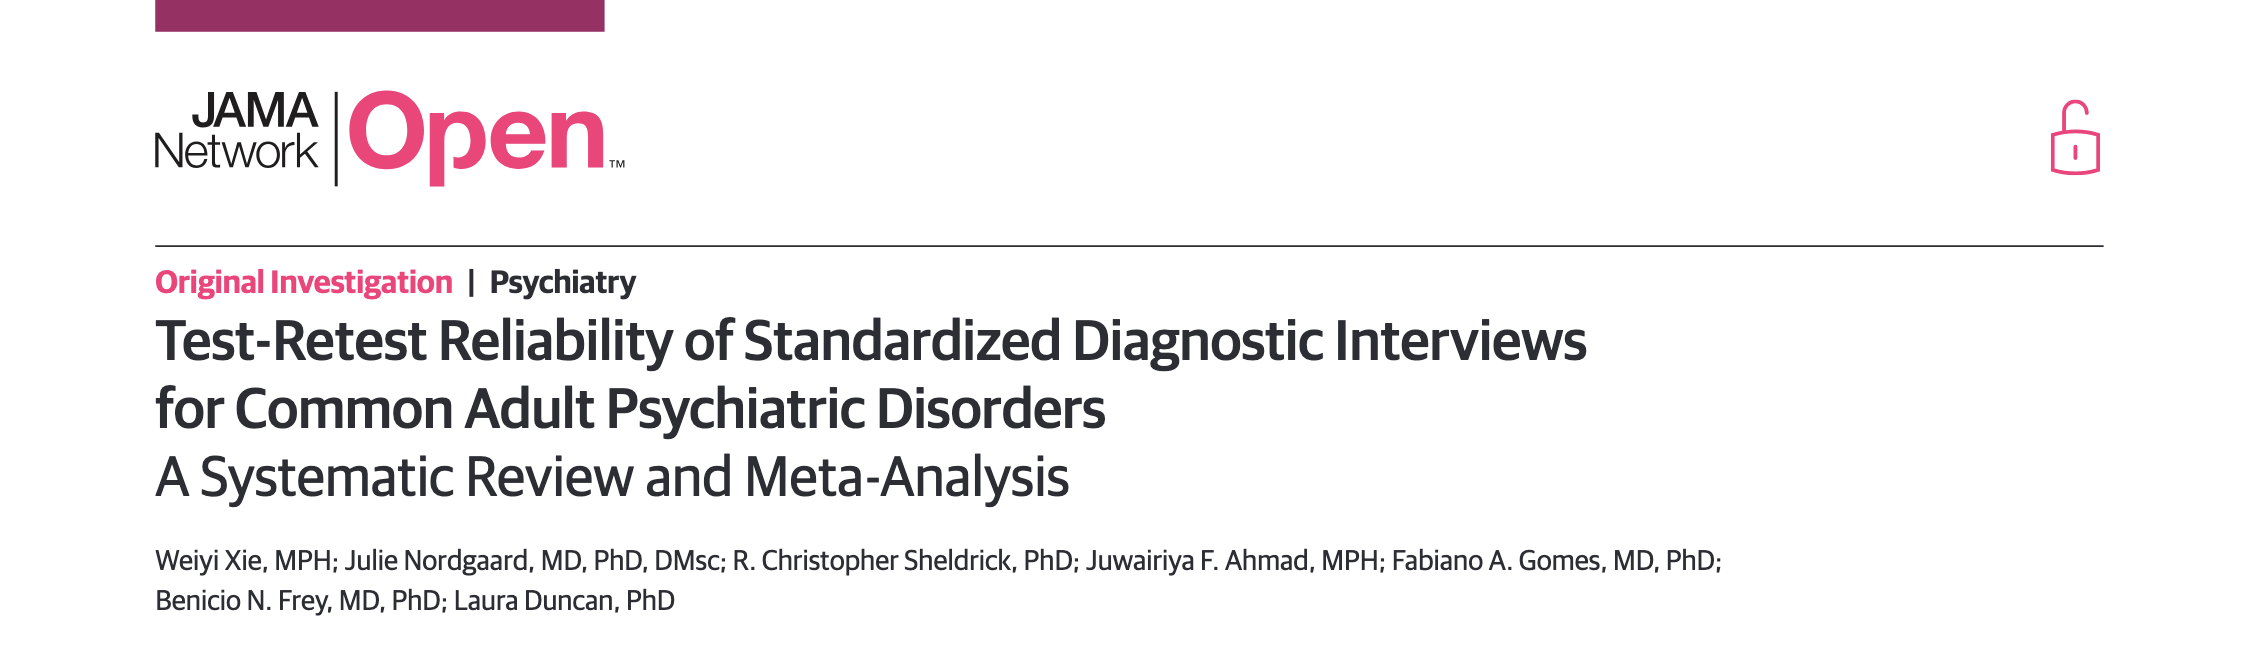
\includegraphics[width=0.95\textwidth]{Figures/Xie_JAMA_test_retest.png}
\end{figure}
\vfill
\end{frame}

\begin{frame}{Affidabilità Split-Half}
\phantomsection\label{affidabilituxe0-split-half}
L'affidabilità split-half stima l'affidabilità di un test misurando la
correlazione tra due metà del test (tipicamente item pari vs item
dispari).

Poiché ciascuna metà è più corta del test intero, la correlazione tra le
metà sottostima l'affidabilità del test completo: si applica quindi la
\textbf{correzione di Spearman-Brown}.

Valori maggiori a 0.70-0.80 sono desiderabili.
\end{frame}

\begin{frame}{Affidabilità Split-Half}
\phantomsection\label{affidabilituxe0-split-half-1}
L'affidabilità Split-half è meno dispendiosa da calcolare rispetto a
quella test-retest.

Il principale limite è che il risultato dipende molto dalla divisione
nelle metà (arbitraria.)
\end{frame}

\begin{frame}{Consistenza interna}
\phantomsection\label{consistenza-interna}
\textbf{Consistenza interna}: rappresenta la consistenza tra gli item di
un test --- quanto gli item sono coerenti tra loro, cioè misurano in
parte la stessa cosa.

In genere è calcolata tramite l'alpha di Cronbach (media di tutte le
possibili split-half reliability), ma l'\textbf{omega di McDonald} è
oggi considerato un'alternativa più robusta (assume meno vincoli sugli
item). L'alpha resta un \textbf{limite inferiore} della reale
consistenza interna. Nessuna delle due è indicata per test a tempo
(\emph{speed tests}).

valori maggiori a 0.70 sono desiderabili, ma spesso in test
neuropsicologici sono intorno a 0.60.
\end{frame}

\begin{frame}{Variazioni nell'affidabilità}
\phantomsection\label{variazioni-nellaffidabilituxe0}
Come per la validità anche l'affidabilità di una specifica misurazione
può cambiare.

Se cambiano procedure (o se ci sono interferenze) l'affidabilità può
essere inferiore.
\end{frame}

\begin{frame}{Relazione tra Validità e Affidabilità}
\phantomsection\label{relazione-tra-validituxe0-e-affidabilituxe0}
\begin{center}
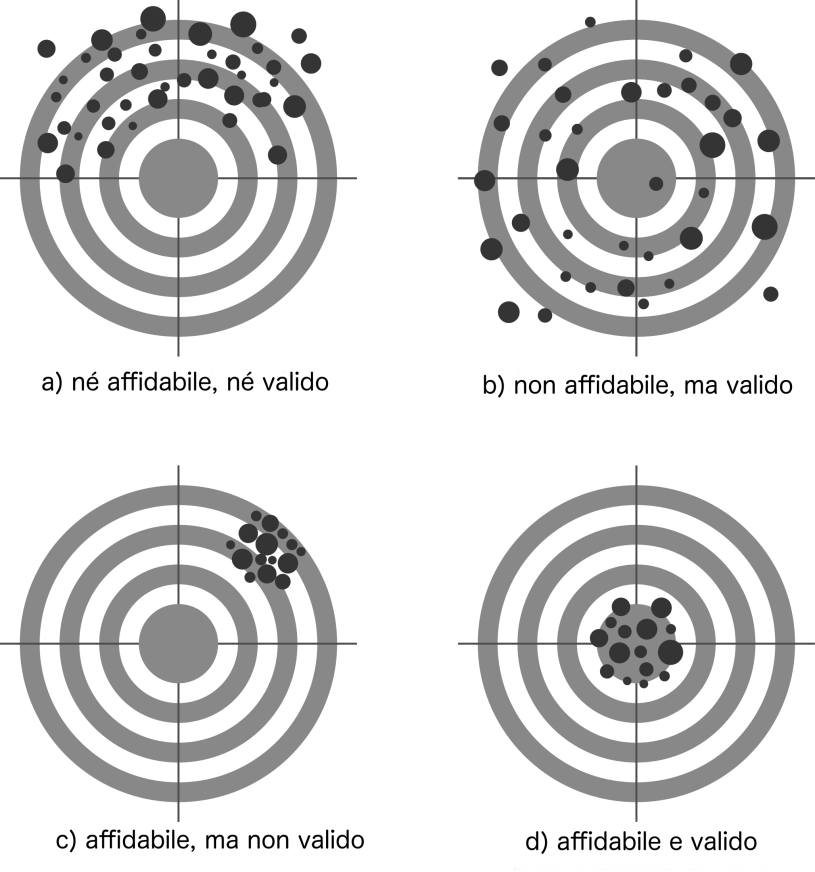
\includegraphics[width=0.5\linewidth,height=\textheight,keepaspectratio]{Figures/Validity_Reliability.png}
\end{center}

\tiny

Figura adattata da ``Reliability and validity'' by © Nevit Dilmen.
Licensed under CC BY-SA 3.0 via Commons.
\end{frame}

\begin{frame}{Validità e affidabilità in pratica}
\phantomsection\label{validituxe0-e-affidabilituxe0-in-pratica}
L'Affidabilità non è solo qualche numero indicato nei manuali dei test,
ma dei valori che hanno un impatto sulle conclusioni cliniche tratte dai
test.
\end{frame}

\begin{frame}{Prove di Validità e affidabilità}
\phantomsection\label{prove-di-validituxe0-e-affidabilituxe0}
\begin{columns}
\column{0.8\textwidth}
\small
Il fatto che un test sia stato pubblicato non ci assicura che sia validato per qualche ragione
 e abbia affidabilità sufficiente! (Disclaimer: Anche test pubblicati da me hanno bassa affidabilità, usare con cautela)

\column{0.2\textwidth}
\begin{figure}
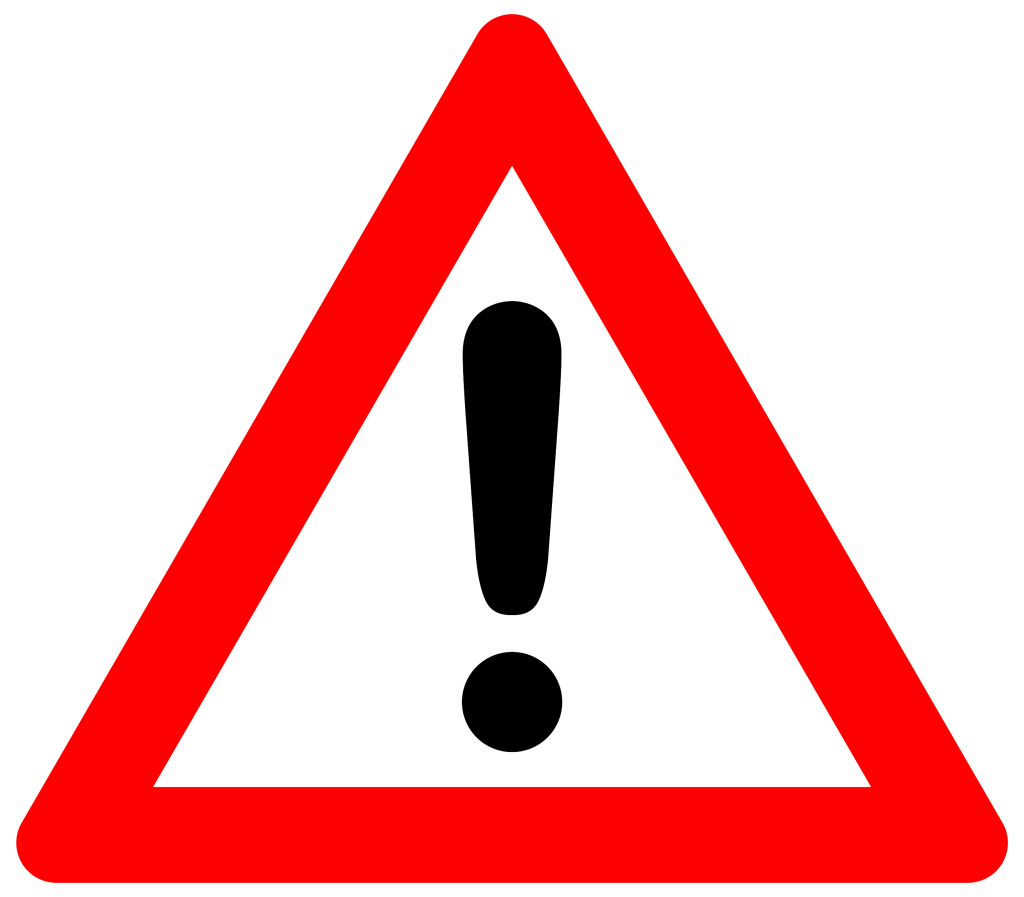
\includegraphics[scale=0.05]{Figures/triangle.png}
\end{figure}
\end{columns}

{\small Da APACS (Arcara \& Bambini, 2016)}
\begin{figure}
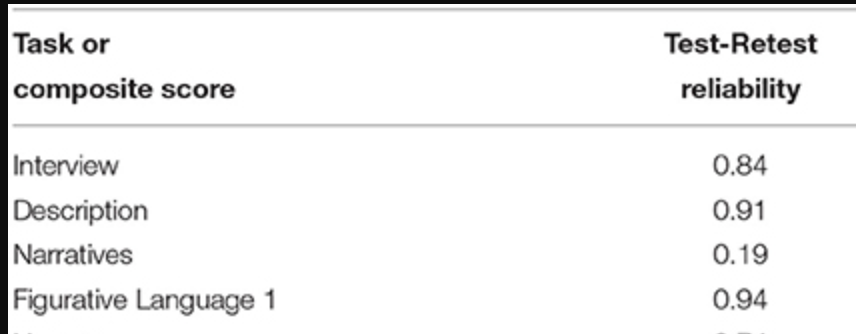
\includegraphics[height=0.5\textheight]{Figures/APACS_reliability.png}
\end{figure}
\end{frame}

\begin{frame}{Validità, affidabilità e invarianza di misura}
\phantomsection\label{validituxe0-affidabilituxe0-e-invarianza-di-misura}
Solitamente informazioni su validità e affidabilità sono disponibili e
ottenute solo su un gruppo di soggetti. Di norma solo su soggetti sani,
ma se sono disponibili dati su pazienti di un certo tipo, solo di un
certo tipo.

Esistono una serie di analisi dette di \textbf{invarianza di misura} che
vanno a valutare se le proprietà di misurazione si mantengono costanti
anche per diversi gruppi.
\end{frame}

\begin{frame}{Effetto di perturbazioni su Validità e Affidabilità.}
\phantomsection\label{effetto-di-perturbazioni-su-validituxe0-e-affidabilituxe0.}
Provate ad immaginare di perturbare una relazione ipoteticamente
perfetta. Che effetti ha su validità ed affidabilità \emph{di una
specifica misura}?

\begin{figure}
  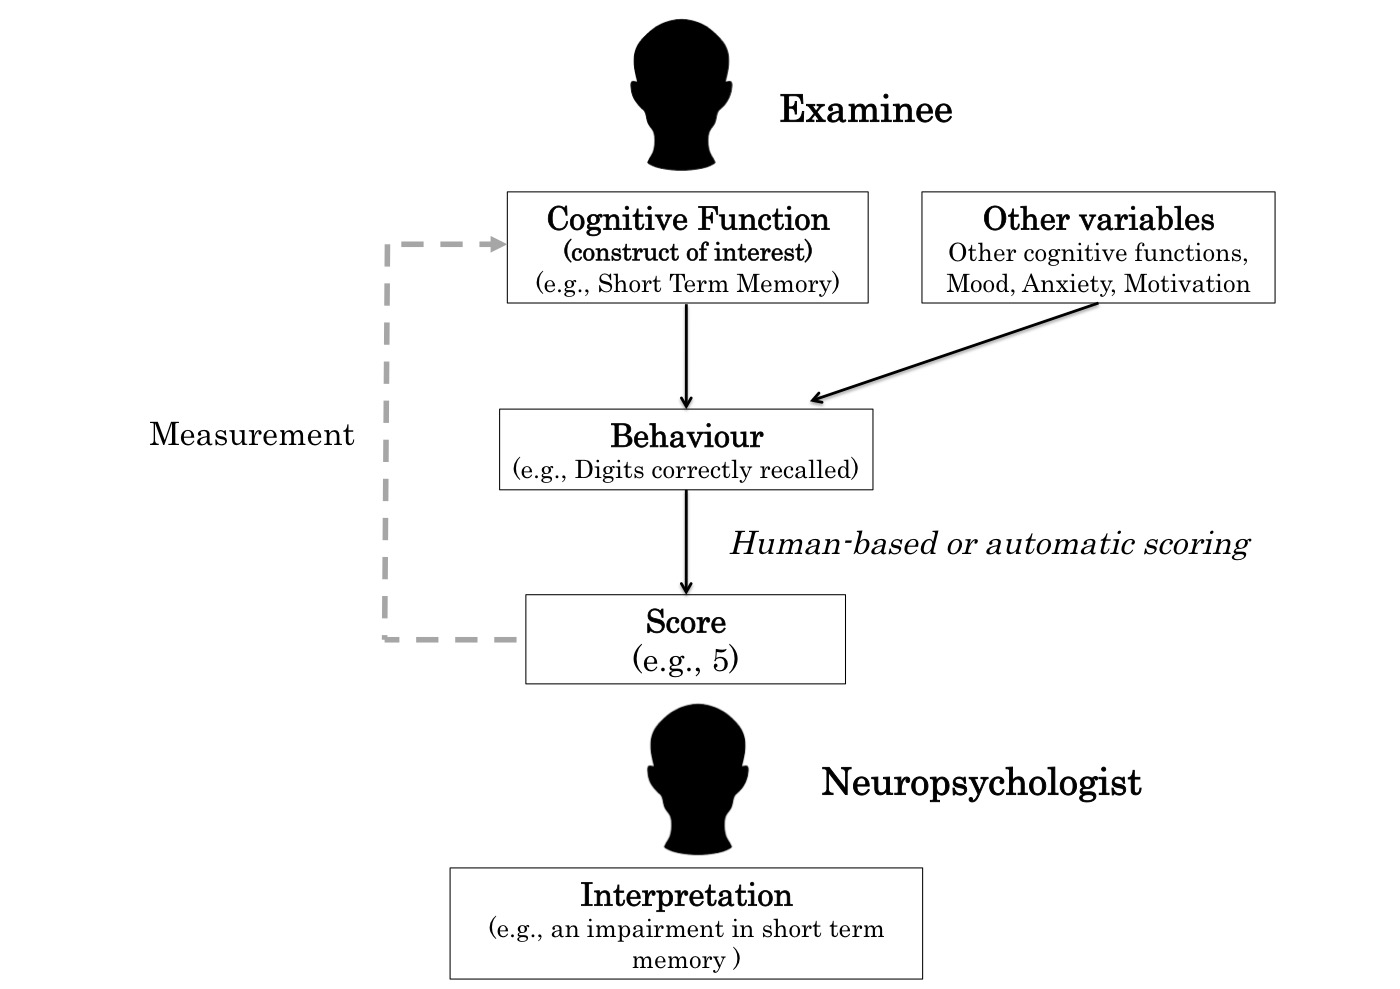
\includegraphics[scale=0.3]{Figures/measurement_diagramma.png}
\end{figure}
\end{frame}

\begin{frame}{Considerazioni conclusive 1/4}
\phantomsection\label{considerazioni-conclusive-14}
Affidabilità e validità sono due qualità importanti che ci permettono di
valutare un test.

In generale, una volta che abbiamo identificato cosa dobbiamo misurare,
dovremmo scegliere test con elevata affidabilità e validità per le
interpretazioni che ci servono
\end{frame}

\begin{frame}{Considerazioni conclusive 2/4}
\phantomsection\label{considerazioni-conclusive-24}
Queste due qualità non ci dicono però necessariamente, l'\textbf{utilità
clinica/forense} del test \textbf{per una specifica valutazione}.

Un test potrebbe essere eccellente per misurare un certo costrutto, ma
poi, in fin dei conti, non aiutarci nella diagnosi dei disturbi di uno
specifico individuo, a fini clinici (es. per diagnosi o lo stabilire il
piano riabilitativo), o rispondere alla nostra specifica domanda
forense.

Ad esempio, se la domanda forense è quantificare un danno di memoria, un
test eccellente per il linguaggio potrebbe non essere utile.
\end{frame}

\begin{frame}{Considerazioni conclusive 3/4}
\phantomsection\label{considerazioni-conclusive-34}
Oltre a questo, Validità e Affidabilità in genere esprimono delle
qualità del test ma non è detto che il test mantenga le stesse qualità
nella specifica misurazione.

Ad esempio se un test ha molte evidenze di validità nel misurare la
memoria, potrebbe poi non farlo più nel corso di una misurazione
specifica (es. perché il paziente non è collaborativo, cerca di simulare
un deficit, non ha compreso le istruzioni, etc.)
\end{frame}

\begin{frame}{Considerazioni conclusive 4/4}
\phantomsection\label{considerazioni-conclusive-44}
Validità e affidabilità vanno sempre considerate come proprietà di un
test \emph{in condizioni ideali}. Anche se un test ha ottimi valori,
potrebbe dare comunque risultati completamente inesatti se usato in
maniera inappropriata o se ci sono circostanze esterne negative (es. chi
è esaminato non è collaborante).

Una delle critiche della definizione fornita di Validità è infatti non
stressare il fatto che è la misurazione ad essere valida o meno (più che
il test).

In ambito forense l'identificazione di ``simulatori'' (capitolo separato
di questo corso) si focalizza proprio sull'identificare la validità
\emph{di specifiche valutazioni}.
\end{frame}

\section{Riferimenti}\label{riferimenti}

\begin{frame}{Riferimenti}
\phantomsection\label{riferimenti-1}
\footnotesize

\begin{itemize}
\tightlist
\item
  AERA, APA, \& NCME (2014). \emph{Standards for Educational and
  Psychological Testing.}
\item
  Cicchetti, D. V., \& Sparrow, S. S. (1981). Developing criteria for
  establishing interrater reliability of specific items.
\item
  Fastenau, P. S., et al.~(1996). Interrater reliability of standard and
  alternate versions of the Complex Figure Test.
\item
  Slick, D. J. (2006). Psychometrics in neuropsychological assessment
  (cap. 1 in Spreen \& Strauss, 2006).
\item
  Lago, S., Bevilacqua, F., Stabile, M. R., Scarpazza, C., Bambini, V.,
  \& Arcara, G. (2022). Case report: Pragmatic impairment in multiple
  sclerosis after worsening of clinical symptoms. \emph{Frontiers in
  Psychology}.
\item
  Arcara, G., \& Bambini, V. (2016). A test for the assessment of
  pragmatic abilities and cognitive substrates (APACS).
\end{itemize}
\end{frame}




\end{document}
